\documentclass[12pt]{article}
\usepackage[margin=1in]{geometry} 
\usepackage{amsmath,amsthm,amssymb,amsfonts}
\usepackage{enumerate,listings,graphicx,epstopdf,siunitx}
\usepackage{color}
\graphicspath{~/Documents/school/fall16/stat586/hw6}
\setcounter{secnumdepth}{0}

\sloppy
\definecolor{lightgray}{gray}{0.5}
 
\newcommand{\N}{\mathbb{N}}
\newcommand{\Z}{\mathbb{Z}}
\newcommand{\normD}[3]{\frac{1}{\sqrt{2\pi #1^2}}exp\left(\frac{-( #2 - #3)^2}{2 #1^2}\right)} 
\newcommand{\cProb}[2]{P(#1|#2)}
\newcommand{\infInt}{\int_{-\infty}^{\infty}}

\begin{document}
\title{Homework Set 6}
\author{Taylor Bodin}
\maketitle

\section{5.21}
Since the given PDF given is jointly gaussian, it is possible to set up a system of equations to find
the mean and variance of the marginals, which are also gaussian distributed. Solving that system gives
the following values:
\[\rho_{xy} = -\frac{1}(2), \sigma_x = -1, \sigma_y = -2, \mu_x = \mu_y = 0\]

\subsection{a.}
\begin{align*}
  f_x(x) &= \normD{(-1)}{x}{0} \\
  f_y(y) &= \normD{(-2)}{y}{0}
\end{align*}

\subsection{b.}
\begin{align*}
  E[X] &= E[Y] = 0 \\
  \sigma_X^2 &= 4 \\ 
  \sigma_Y^2 &= 1 \\ 
\end{align*}

\subsection{c.}
\begin{align*}
  f_{x|y}(x|y) &= \frac{f_{x,y}(x,y)}{f_y(y)} \\
  &= \frac{\frac{1}{2\pi\sqrt{3}}exp\left( -\frac{x^2 + 2xy + 4y^2}{6} \right)}
    {\frac{1}{\sqrt{2\pi}}exp\left( -\frac{y^2}{2} \right)} \\
    &= \frac{\sqrt{6}}{6\sqrt{\pi}}exp\left( -\frac{x^2 + 2xy + y^2}{6} \right)
\end{align*}

\subsection{d.}
\begin{align*}
  \rho_{x,y} &= \frac{-1}{2} \\
  Cov(x,y) &= \sigma_x \sigma_y \rho_{xy} = -1 \\
  E[XY] &= Cov(x,y) + \mu_x \mu_y = -1
\end{align*}

\section*{Problem 5.25}
\subsection*{a.}
\begin{align*}
  E[U] &= E[X+2Y] = E[X] + 2E[Y] = \mu_x + 2\mu_y = 0 \\
  E[V] &= E[X+2Y] = 2E[X] - E[Y] = 2\mu_x - \mu_y = 3 \\
\end{align*}

\subsection*{b.}
First we have to do some ground work:
\begin{align*}
  E[U^2] &= E[(X+2Y)^2] = E[X^2] + 4E[XY] + 4E[Y^2] \\
  E[X^2] &= \sigma_x^2 + \mu_x^2 = 5 \\
  E[Y^2] &= \sigma_y^2 + \mu_y^2 = 17 \\
  E[XY] &= Cov(X,Y) + \mu_x \mu_y = -1 \\
  Cov(X,Y) &= \rho_{XY}\sigma_x \sigma_y = 1 \\
  E[U^2] &= E[(X+2Y)^2] = E[X^2] + 4E[XY] + 4E[Y^2] = 5 + -4 + 4(17) = 69 \\
  E[V^2] &= E[(2X-Y)^2] = 4E[X^2] -4E[XY] + E[Y^2] = 4(5) + 4 + 17 = 41 \\
  \sigma_U^2 &= E[U^2] - E[U]^2 = 69 - 0 = 69 \\ 
  \sigma_V^2 &= E[V^2] - E[V]^2 = 41 - 3 = 38 \\ 
\end{align*}

\subsection{c.}
\begin{align*}
  E[UV] &= E[(X+2Y)(2X-Y)] = 2E[X^2] + 3E[XY] - 2E[Y^2] \\
  &= 2(5) + 3(-1) - 2(17) = -27 \\
  Cov(U,V) &= E[UV] - E[U]E[V] = -27 - 0 = -27 \\
  \rho_{UV} &= \frac{Cov(U,V)}{\sqrt{Var(U)Var(V)}} = \frac{-27}{\sqrt{69(38)}} = -.5273
\end{align*}

\section{Problem 5.29}
\subsection{a.}
These two RV will be orthogonal when their inner product is 0:

\begin{align*}
  0 &= \frac{1}{(2\pi)^2}\int_0^{2\pi} cos(a\theta)sin(a\theta) d\theta \\
  &= -\frac{1}{(2\pi)^2}\frac{cos^2(a\theta)}{2a}\big|_0^{2\pi} \\
  &= -\frac{1}{(2\pi)^2}\frac{cos^2(a2\pi)}{2a} \\
  &= -\frac{1}{(2\pi)^2}\frac{sin(a2\pi)}{2a} \\
  &= sin(a2\pi) \\
  a &= \frac{sin^{-1}(0)}{2\pi} \\
  a &= \frac{1}{2}n, & & n = 0, 1 , 2 \dots
\end{align*}

\subsection{b.}
\[\int_0^{2\pi} \frac{cos(a\theta)}{2\pi}\frac{sin(a\theta)}{2\pi} d\theta
  = \int_0^{2\pi} \frac{cos(a\theta)}{2\pi}d\theta \int_0^{2\pi}\frac{sin(a\theta)}{2\pi} d\theta \]
This equality holds for all values of a, therefore these RV are uncorrelated.

\section{Problem 5.33}
\subsection{a.}
If X and Y are independent, $P(X=i, Y=j) = P(X=i)P(Y=j)$. Two vectors can then be formed as such,
$\textbf{U}(i) = P(X=i), \textbf{V}(i) = P(Y=j)$. Finally, the outer product of these two vectors 
forms a matrix which is the joint PMF:
\[
  \textbf{U} \otimes \textbf{V} =
\begin{bmatrix}
    U_1V_1 & U_1V_2 & U_1V_3 & \dots  & U_1V_k \\
    U_2V_1 & U_2V_2 & U_2V_3 & \dots  & U_2V_k \\
    \vdots & \vdots & \vdots & \ddots & \vdots \\
    U_kV_1 & U_kV_2 & U_kV_3 & \dots  & U_kV_k
\end{bmatrix}
= P(X=i, Y=j)
\]

\subsection{b.}
The converse is also true because the outer produce is a linear operator and therfore, the joint distribution
can be mapped back and forth using the relationship above. In other words, if the the two RV that make up a joint
are independent, the joint PMF can be decomposed into the two vectors mentioned above which represent the marginal
PMFs. 

\section{Problem 5.37}
\subsection{a.}
\[
  f_{x,y}(x,y) = \frac{\sqrt{15}}{30\pi}
  exp\left( -\left[ \frac{(\frac{x-2}{1})^2+\frac{1}{2}\frac{x-2}{1}\frac{y+3}{4} + (\frac{y+3}{4})^2}{\frac{15}{8}} \right] \right)
\]

\subsection{b.}
\begin{align*}
  f_X(x) &= \frac{1}{\sqrt{2\pi}}exp\left( -\frac{(x-2)^2}{2} \right) \\
  f_Y(x) &= \frac{1}{\sqrt{32\pi}}exp\left( -\frac{(y+3)^2}{32} \right)
\end{align*}

\subsection{c.}
\begin{align*}
  P(X<0) &= 1 - Q\left( \frac{0-\mu_x}{\sigma_x} \right) = 1 - Q(-2) \\
  P(Y>0) &= Q\left( \frac{0-\mu_y}{\sigma_y} \right) = 1 - Q\left(\frac{3}{4}\right) \\
\end{align*}

\section{Problem 5.41}
\begin{align*}
  \Theta_{X,Y}(\omega_1,\omega_2) &= E\left[ exp(j\omega_2 Y)E[exp(j\omega_1X|y)] \right] \\
  &= E\left[ exp(j\omega_2 Y)\left( exp(j(\mu_{x|y}\omega_1)-\frac{\omega_1^2\sigma_{x|y}^2)}{2} \right)\right] \\
  &= exp\left( -\frac{\omega_1^2(\sigma_x^2(1-\rho_{xy}^2)^2)}{2} \right)
  exp\left( -\omega_1(\mu_X+\rho_{XY})(\frac{\sigma_x}{\sigma_y}) \right)
  E\left[exp\left( jY(\omega_2+(\mu_x+\rho_{xy})\frac{\sigma_x}{\sigma_y}\omega_1)\right)\right] \\
  &= exp\left( -\frac{\omega_1^2(\sigma_x^2(1-\rho_{xy}^2)^2)}{2} 
  -\omega_1(\mu_X+\rho_{XY})(\frac{\sigma_x}{\sigma_y})
  -\frac{(\omega_2+(\mu_x+\rho_{xy})\frac{\sigma_x}{\sigma_y}\omega_1)^2-\mu_y}{2\sigma_Y}\right) \\
\end{align*}

\section{Problem 5.45}
\subsection{a.}
\begin{align*}
  E[M] &= \frac{\delta H(z_1,z_2}{\delta z_1}\big|_{z_1 = z_2 = 1} = \frac{8}{4-z1-z2} = 1 \\
  E[N] &= \frac{\delta H(z_1,z_2}{\delta z_2}\big|_{z_1 = z_2 = 1} = \frac{8}{4-z1-z2} = 1 \\
\end{align*}

\subsection{b.}
\[
E[MN] = \frac{\delta H(z_1,z_2}{\delta z_1 \delta z_2}\big|_{z_1 = z_2 = 1} = \frac{24}{4-z1-z2} = \frac{3}{2}
\]

\subsection{c.}
\begin{align*}
  P_{X,Y}(k,1) &= \frac{1}{k!l!} \frac{\delta^k \delta^l}{\delta z_1^k \delta z_2^l} H_{X,Y}(z_1,z_2)\big|_{z_1=z_2=0} \\
  &= \frac{\frac{1}{4}}{(1-\frac{z_1+z_2}{4})^2} \\
  &= \frac{1}{4} \sum_{k=1}^\infty k \left(\frac{z_1+z_2}{4}\right)^{k-1} \\
  &= \frac{1}{4} \sum_{p=0}^\infty (p+1) \left(\frac{z_1+z_2}{4}\right)^p \\
  \therefore \\
  P_{M,N}(m,n) &= \frac{m+n+1}{4(m+n+1)} \binom{m+n}{n}, & & n,m = 0 , 1 , 2 \dots
\end{align*}

\section{Problem 5.49}
\begin{align*}
f_Z(z) &= f_X(z) * f_Y(z) \\
&= \int_{-\infty}^\infty f_X(z-y)(-f_Y(z))dy \\
&= -ab\int_{-\infty}^\infty exp(-a(z-y))exp(-by)u(z-y)u(y)dy \\
&= -abexp(-az)\int_{0}^z exp((a-b)y)dy \\
&= \frac{-abexp(-az)}{a-b}\left[ exp((a-b)y)\big|_0^z \right] \\
&= \frac{-ab}{a-b}\left[ exp(-bz)-exp(-az) \right], & & b>a
\end{align*}

\section{Problem 5.53}
I attempted this one, but I ran into some problems. I could try to convolve these pdfs to determine the pdf of z, but that intergral
doesn't look very solvable. Then I thought I could multiple the characeristic function of a Rayleigh by the CF of a arcsine, which
is doable, but then doing the inverse transform looked daunting. Finally, I don't understand the conditional PDF approach since,
it seems to imply that I already have $f_z(z)$ to condition on. 
\section{Problem 5.57}
\begin{align*}
  E[U] &= aE[X] + bE[Y] = 0 \\
  E[V] &= cE[X] + dE[Y] = 0 \\
  E[UV] &= acE[X^2] + bdE[Y^2] + (ad+bc)E[XY] \\
  0 &= ac + bd + (ad+bc)\rho
\end{align*}

\section{Problem 5.61}
\subsection{a.}
\begin{align*}
  P_M(k) &= P_N(k) = \frac{1}{k}, & & k = 0,1,2 \dots k-1 \\
  P_L(k) &= \sum_p P_M(k-p)P_N(p) \\
  &= \sum_{i=0}^k \frac{1}{k^2} \\
  &= \frac{k+1}{k^2}
\end{align*}

\subsection{b.}
\begin{align*}
  P_M(m) &= (1-p)p^m, & &  m = 0,1,2,\dots \\
  P_N(n) &= (1-q)q^n, & &  n = 0,1,2,\dots \\
  P_L(k) &= \sum_p P_M(k-p)P_N(p) \\
  &= \sum_{i=0}^k (1-p)p^{k-i}(1-q)q^i \\
  &= (1-p)(1-q)p^k\sum_{p=0}^k p^{-i}q^i \\
  &= (1-p)(1-q)p^k\sum_{p=0}^k \left( \frac{q}{p} \right)^i \\
  &= (1-p)(1-q)p^k \frac{1-\left(\frac{q}{p}\right)^{k+1}}{1-\frac{q}{p}} \\
  &= (1-p)(1-q) \frac{p^{k+1}-q^{k+1}}{p-q}
\end{align*}

\subsection{c.}
\begin{align*}
  P_M(m) &= P_N(m) = (1-p)p^m, & &  m = 0,1,2,\dots \\
  P_L(k) &= \sum_p P_M(k-p)P_M(p) \\
  &= \sum_{i=0}^k (1-p)p^{k-i}(1-p)p^i \\
  &= (1-p)^2p^k\sum_{i=0}^k p^{-i}p^i \\
  &= (1-p)^2p^k(k+1)
\end{align*}

\section*{Problem 5.79}

\begin{par}
I copied the code from example 5.16 and made one change to meet the requirments for this part
\end{par} \vspace{1em}

\subsection*{Contents}

\begin{itemize}
\setlength{\itemsep}{-1ex}
   \item Setup
   \item Generate the RVs and count
   \item Plot
\end{itemize}


\subsection*{Setup}

\begin{verbatim}
clear
N=1000; % number of samples per iteration
bw=0.1; % bin widths for histogram
xbins=[-1.4:bw:1.4];
ybins=[-1.4:bw:1.4]; % histogram bins
iterations=100; % number of iterations
M=length(xbins);
Nsamples=zeros(M); % initialize matrix for storing data
count=0; % initialize counter.
\end{verbatim}


\subsection*{Generate the RVs and count}

\begin{verbatim}
for ii=1:iterations
x=2*rand(1,N)-1; y=2*rand(1,N)-1; % generate variables over square
% keep only those within the unit circle.
X=[]; Y=[];
for k=1:N
if x(k)^2+4*y(k)^2<1
X=[X x(k)];
Y=[Y y(k)];
end % end if statement
end % end k loop
count=count+length(X); % count random samples generated
% Compute number of samples that fall within each bin.
for m=1:length(xbins)
for n=1:length(ybins)
temp1=(abs(X-xbins(m))<bw/2);
temp2=(abs(Y-ybins(n))<bw/2);
Nsamples(m,n)=Nsamples(m,n)+sum(temp1.*temp2);
end % end n loop
end % end m loop
end % end iterations
\end{verbatim}


\subsection*{Plot}

\begin{verbatim}
PDFest=Nsamples/(count*bw^2); % convert to prob. densities
mesh(xbins,ybins,PDFest) % plot estimate of joint PDF
xlabel('x'); ylabel('y'); % label plot axes
zlabel('Joint PDF');
\end{verbatim}

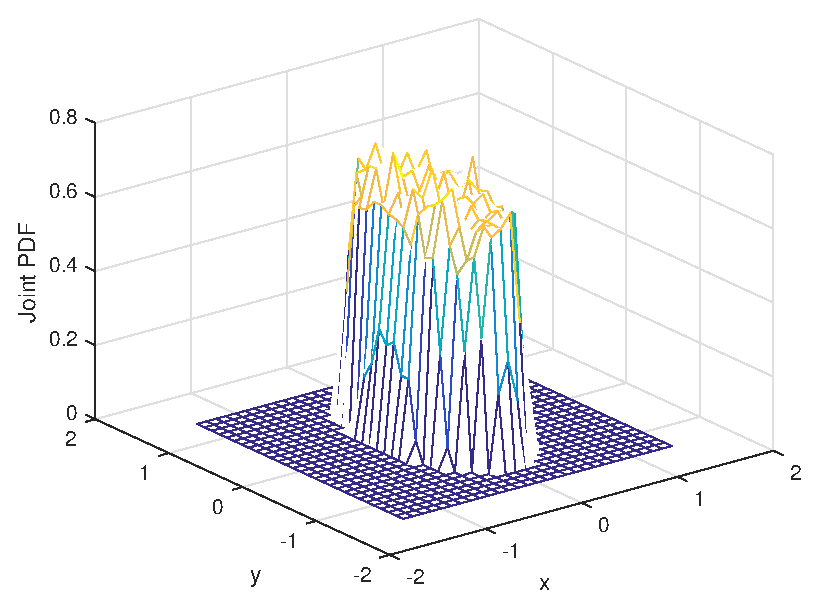
\includegraphics [width=4in]{prob_5_79_01.eps}




\end{document}

